\documentclass[a4paper, 12pt]{report}

% Packages
\usepackage[protrusion=false]{microtype}
\usepackage{setspace}

% Language Package
\usepackage[hidelinks]{hyperref}
\usepackage[italian]{babel}
\usepackage[italian]{cleveref}
\usepackage[toc,page]{appendix}
\usepackage{graphicx}
\usepackage[font=footnotesize,labelfont=bf]{caption}

% Environments
\newenvironment{packed_enum}{
\begin{enumerate}
        \setlength{\itemsep}{1pt}
        \setlength{\parskip}{0pt}
        \setlength{\parsep}{0pt}
}{\end{enumerate}}

\newenvironment{packed_itemize}{
\begin{itemize}
        \setlength{\itemsep}{1pt}
        \setlength{\parskip}{0pt}
        \setlength{\parsep}{0pt}
}{\end{itemize}}

% Initialization
\title{Relazione Progetto HPC 2023}
\author{Michele Montesi \\
        Matricola: 0000974934 \\
        E-Mail: michele.montesi3@studio.unibo.it}

\date{\today}

\begin{document}
\maketitle
% \tableofcontents

\chapter*{Introduzione}
\begin{sloppypar}
La presente ricerca presenta lo sviluppo di due versioni parallelizzate del software \texttt{sph.c}, 
implementate utilizzando la libreria \texttt{OpenMP} e la libreria \texttt{MPI} rispettivamente. 
L'obiettivo della ricerca è quello di valutare i vantaggi prodotti dall'utilizzo della programmazione multi-processore.
\end{sloppypar}

\bigskip

\begin{sloppypar}
\noindent
Per misurare le prestazioni del software in questione è stato creato uno script python che lo esegue, incrementando
il numero di threads partendo da 1 fino a 12 e il numero di particelle da 1400 a 5700.
Lo script trascrive su un foglio excel i seguenti dati interessati.
Da questi dati viene poi calcolata la media.
\end{sloppypar}

{\let\clearpage\relax\chapter*{Versione OpenMP}}
\section*{Implementazione}
\begin{sloppypar}
  \noindent
  In questa implementazione del software, effettuata con \textit{OpenMP}, sono stati parallelizzati attraverso 
  \texttt{\#pragma omp parallel for}, i cicli delle funzioni indicate.

  \smallskip
  \noindent
  Quando necessario sono state effetuate riduzioni così da rendere più efficiente l'esecuzione del software parallelizzato.
\end{sloppypar}

\section*{Prestazioni}
\subsection*{Raccolta dei dati}
\begin{sloppypar}
  \noindent
  Per misurare le prestazioni del software in questione è stato creato uno script python che lo esegue, incrementando
  il numero di threads partendo da 1 fino a 12 e il numero di particelle da 1400 a 5700.
  Lo script trascrive su un foglio excel i seguenti dati interessati.
  Da questi dati viene poi calcolata la media.
\end{sloppypar}

\subsection*{Valutazione}
\begin{sloppypar}
  \noindent
  Dalla figura \ref{fig:omp_speedup} si nota come lo \texttt{speedup}, all'aumentare del numero di threads, cresca linearmente fino
  a 11, dove raggiunge il suo massimo, diminuendo, poi, a 12. Questo comportamento indica che 11 è il numero di threads
  oltre il quale la parallelizzazione OMP diventa inefficiente.

  \begin{figure}[ht]
    \centering
    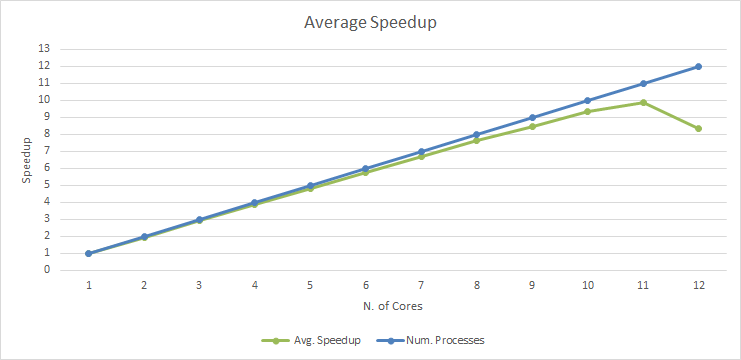
\includegraphics[width=9cm]{img/omp-speedup.png}
    \caption{OpenMP implementation's average speedup}
    \label{fig:omp_speedup}
  \end{figure}

  \noindent
  Dal grafico in figura \ref{fig:omp_sse} si osserva che l'efficienza resta approssimativamente la stessa tra 2 e 10 threads,
  diminuendo di poco con 11 e di molto con 12. La \textit{Strong Scaling Efficiency} indica come all'aumentare dei threads,
  per uno stesso carico di lavoro, il tempo diminuisca. In questo caso fino a 11 threads l'efficienza è ragionevole.

  \begin{figure}[ht]
    \centering
    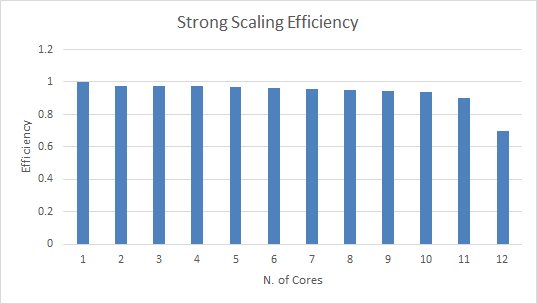
\includegraphics[width=9cm]{img/omp-sse.png}
    \caption{OpenMP implementation's average strong scaling efficiency}
    \label{fig:omp_sse}
  \end{figure}

  \bigskip
  \noindent
  Nella figura \ref{fig:omp_wse} viene esposto l'andamento della \textit{Weak Scaling Efficiency}, la quale
  all'aumentare dei processori aumenta la quantità di lavoro proporzionalmente, in modo da considerare se i
  problemi con più threads vengono risolti nello stesso tempo del problema lineare. In questo caso fino a 11
  threads il tempo è all'incirca lo stesso, mentre con 12 il tempo aumenta.

  \begin{figure}[ht]
    \centering
    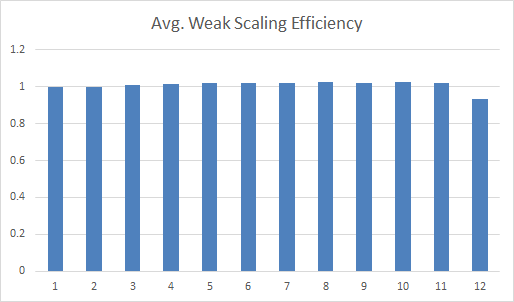
\includegraphics[width=9cm]{img/omp-wse.png}
    \caption{OpenMP implementation's average weak scaling efficiency}
    \label{fig:omp_wse}
  \end{figure}
\end{sloppypar}

{\let\clearpage\relax\chapter*{Versione MPI}}
\section*{Implementazione}
Per l'implementazione del software con \texttt{MPI} è stato creato un \texttt{MPI\_Datatype} contiguo per incapsulare la struttura
dati durante lo scambio di messagi. Per suddividere le particelle fra tutti i processori viene fatta una \texttt{MPI\_Scatterv} dal processo 0.
Dopo \texttt{compute\_density\_pressure} e \texttt{integrate} viene chiamata una \texttt{MPI\_Allgatherv} per raccogliere i dati elaborati
e ridistribuirli nuovamente a tutti i processori mentre per \texttt{compute\_forces} non viene fatto in quanto questo agisce solamente in locale.
Alla fine, dopo aver calcolato la velocità media delle particelle locali, viene eseguita una \texttt{MPI\_Reduce} con operatore somma.
Questo risultato viene diviso per tutti i processi ottenendo così la velocità media complessiva.

\section*{Prestazioni}


\chapter*{Conclusioni}

\end{document}